% Copyright 2020  Ed Bueler

\documentclass[10pt,hyperref,dvipsnames]{beamer}

\mode<presentation>{
  \usetheme{Madrid}
  \usecolortheme{beaver}
  \setbeamercovered{transparent}  
  \setbeamerfont{frametitle}{size=\large}
}

\setbeamercolor*{block title}{bg=red!10}
\setbeamercolor*{block body}{bg=red!5}

\usepackage[english]{babel}
\usepackage[latin1]{inputenc}
\usepackage{times}
\usepackage[T1]{fontenc}
% Or whatever. Note that the encoding and the font should match. If T1
% does not look nice, try deleting the line with the fontenc.

\usepackage{empheq}
\usepackage{xspace}
\usepackage{verbatim,fancyvrb}

\usepackage{tikz}
\usetikzlibrary{shapes,arrows.meta,decorations.markings,decorations.pathreplacing,fadings,positioning}

\usepackage{hyperref}

\newcommand{\ba}{\mathbf{a}}
\newcommand{\bb}{\mathbf{b}}
\newcommand{\bc}{\mathbf{c}}
\newcommand{\bbf}{\mathbf{f}}
\newcommand{\bg}{\mathbf{g}}
\newcommand{\bn}{\mathbf{n}}
\newcommand{\bq}{\mathbf{q}}
\newcommand{\br}{\mathbf{r}}
\newcommand{\bx}{\mathbf{x}}
\newcommand{\by}{\mathbf{y}}
\newcommand{\bv}{\mathbf{v}}
\newcommand{\bu}{\mathbf{u}}
\newcommand{\bw}{\mathbf{w}}

\newcommand{\bF}{\mathbf{F}}
\newcommand{\bG}{\mathbf{G}}
\newcommand{\bQ}{\mathbf{Q}}
\newcommand{\bU}{\mathbf{U}}

\newcommand{\grad}{\nabla}
\newcommand{\Div}{\nabla\cdot}
\newcommand{\minmod}{\operatorname{minmod}}

\newcommand{\CC}{\mathbb{C}}
\newcommand{\RR}{\mathbb{R}}

\newcommand{\ddt}[1]{\ensuremath{\frac{\partial #1}{\partial t}}}
\newcommand{\ddx}[1]{\ensuremath{\frac{\partial #1}{\partial x}}}
\newcommand{\Matlab}{\textsc{Matlab}\xspace}
\newcommand{\Octave}{\textsc{Octave}\xspace}
\newcommand{\eps}{\epsilon}

\newcommand{\ip}[2]{\left<#1,#2\right>}

\newcommand{\xiphalf}{{x_{i+\frac{1}{2}}}}
\newcommand{\ximhalf}{{x_{i-\frac{1}{2}}}}
\newcommand{\Fiphalf}{{F_{i+\frac{1}{2}}}}
\newcommand{\Fimhalf}{{F_{i-\frac{1}{2}}}}
\newcommand{\Fiphalfn}{{F^n_{i+\frac{1}{2}}}}
\newcommand{\Fimhalfn}{{F^n_{i-\frac{1}{2}}}}

\newcommand{\trefcolumn}[1]{\begin{bmatrix} \phantom{x} \\ #1 \\ \phantom{x} \end{bmatrix}}
\newcommand{\trefmatrixtwo}[2]{\left[\begin{array}{c|c|c} & & \\ #1 & \dots & #2 \\ & & \end{array}\right]}
\newcommand{\trefmatrixthree}[3]{\left[\begin{array}{c|c|c|c} & & & \\ #1 & #2 & \dots & #3 \\ & & & \end{array}\right]}
\newcommand{\trefmatrixgroups}[4]{\left[\begin{array}{c|c|c|c|c|c} & & & & & \\ #1 & \dots & #2 & #3 & \dots & #4 \\ & & & & & \end{array}\right]}

\newcommand{\blocktwo}[4]{\left[\begin{array}{c|c} #1 & #2 \\ \hline #3 & #4 \end{array}\right]}

\newcommand{\bqed}{{\color{blue}\qed}}
\newcommand{\ds}{\displaystyle}

\newcommand\mynum[1]{{\renewcommand{\insertenumlabel}{#1}%
      \usebeamertemplate{enumerate item} \,}}


\title{Complementarity for glaciers}

\subtitle{How to apply equations for where equations apply}

\author{Ed Bueler}

\institute[UAF]{University of Alaska Fairbanks}

\date{December 2020}


\begin{document}
\beamertemplatenavigationsymbolsempty

\begin{frame}
  \maketitle
\end{frame}

\begin{frame}
  \frametitle{Outline}
  \tableofcontents[hideallsubsections]
\end{frame}


\section{two precise glaciologists}

\begin{frame}{W}

\begin{columns}
\begin{column}{0.5\textwidth}
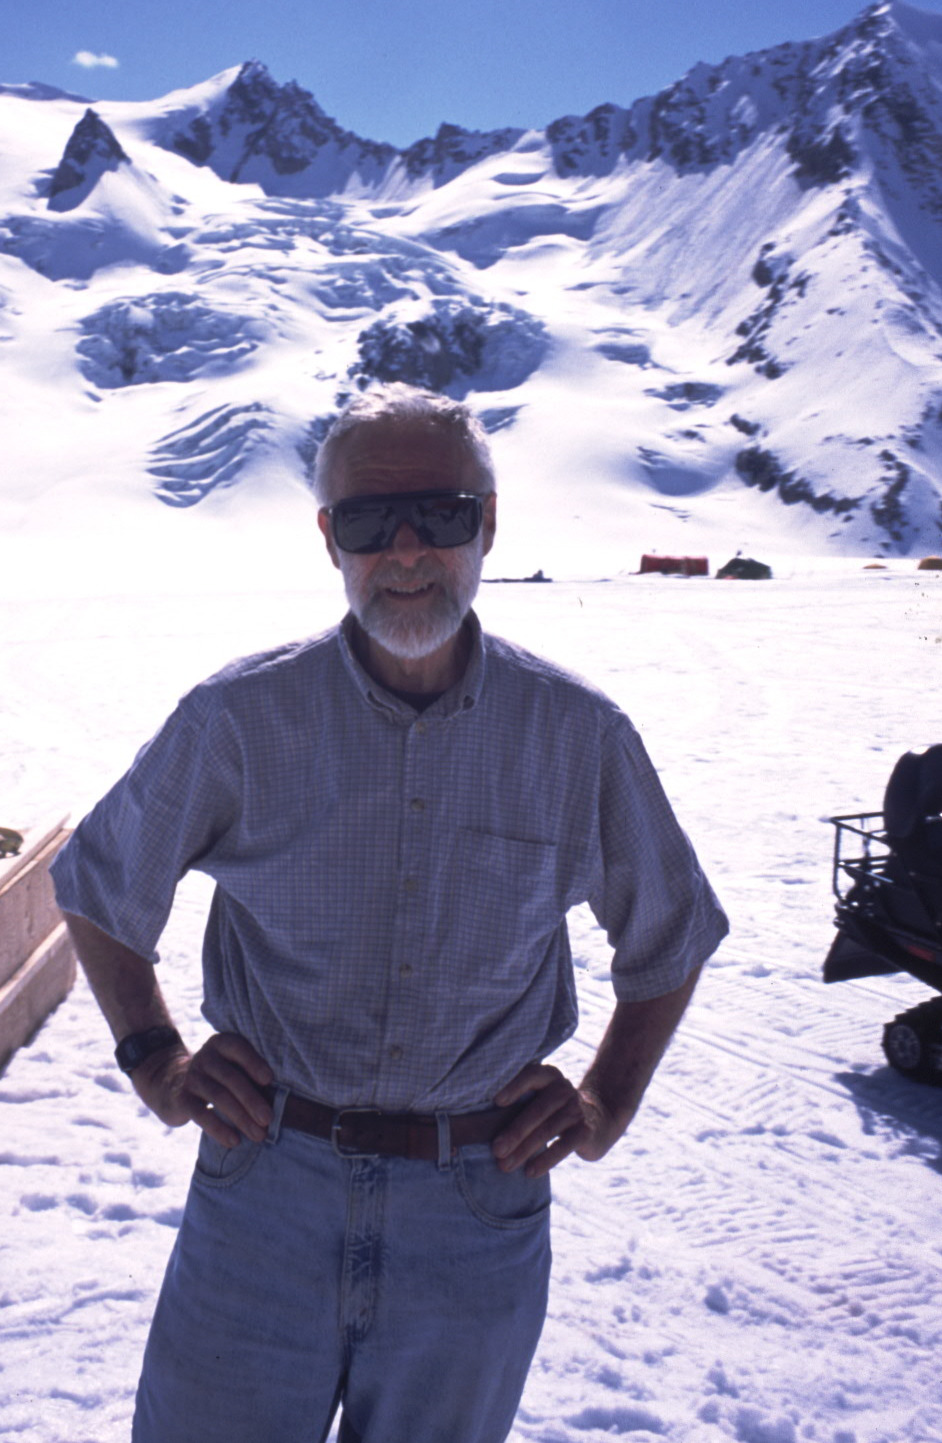
\includegraphics[width=0.8\textwidth]{figs/Will-by-Truffer.jpg}
%\url{https://news.uaf.edu/goodbye-to-a-raffish-glacier-scientist/}

\hfill \tiny \emph{photo by Martin Truffer} \phantom{dklfj asdlfj dslfaj}
\end{column}
\begin{column}{0.5\textwidth}
\begin{itemize}
\item W is a glaciologist
\invisible<1>{\item he is happy because he is standing on a glacier}
\invisible<1-2>{\item he can say two \emph{precise} things about his patch of the world}
\invisible<1-3>{\item one inequality and one equality}
\invisible<1-4>{\item<5>[($>$)] the glacier thickness is positive
    $$H>0$$}

\vspace{-5mm}
\invisible<1-4>{\item<5>[($=$)] the mass of ice is conserved
    $$\frac{\partial H}{\partial t} + \Div \left(\bU H\right) = a$$}
\end{itemize}
\end{column}
\end{columns}
\end{frame}

\begin{frame}{A}

\begin{columns}
\begin{column}{0.5\textwidth}
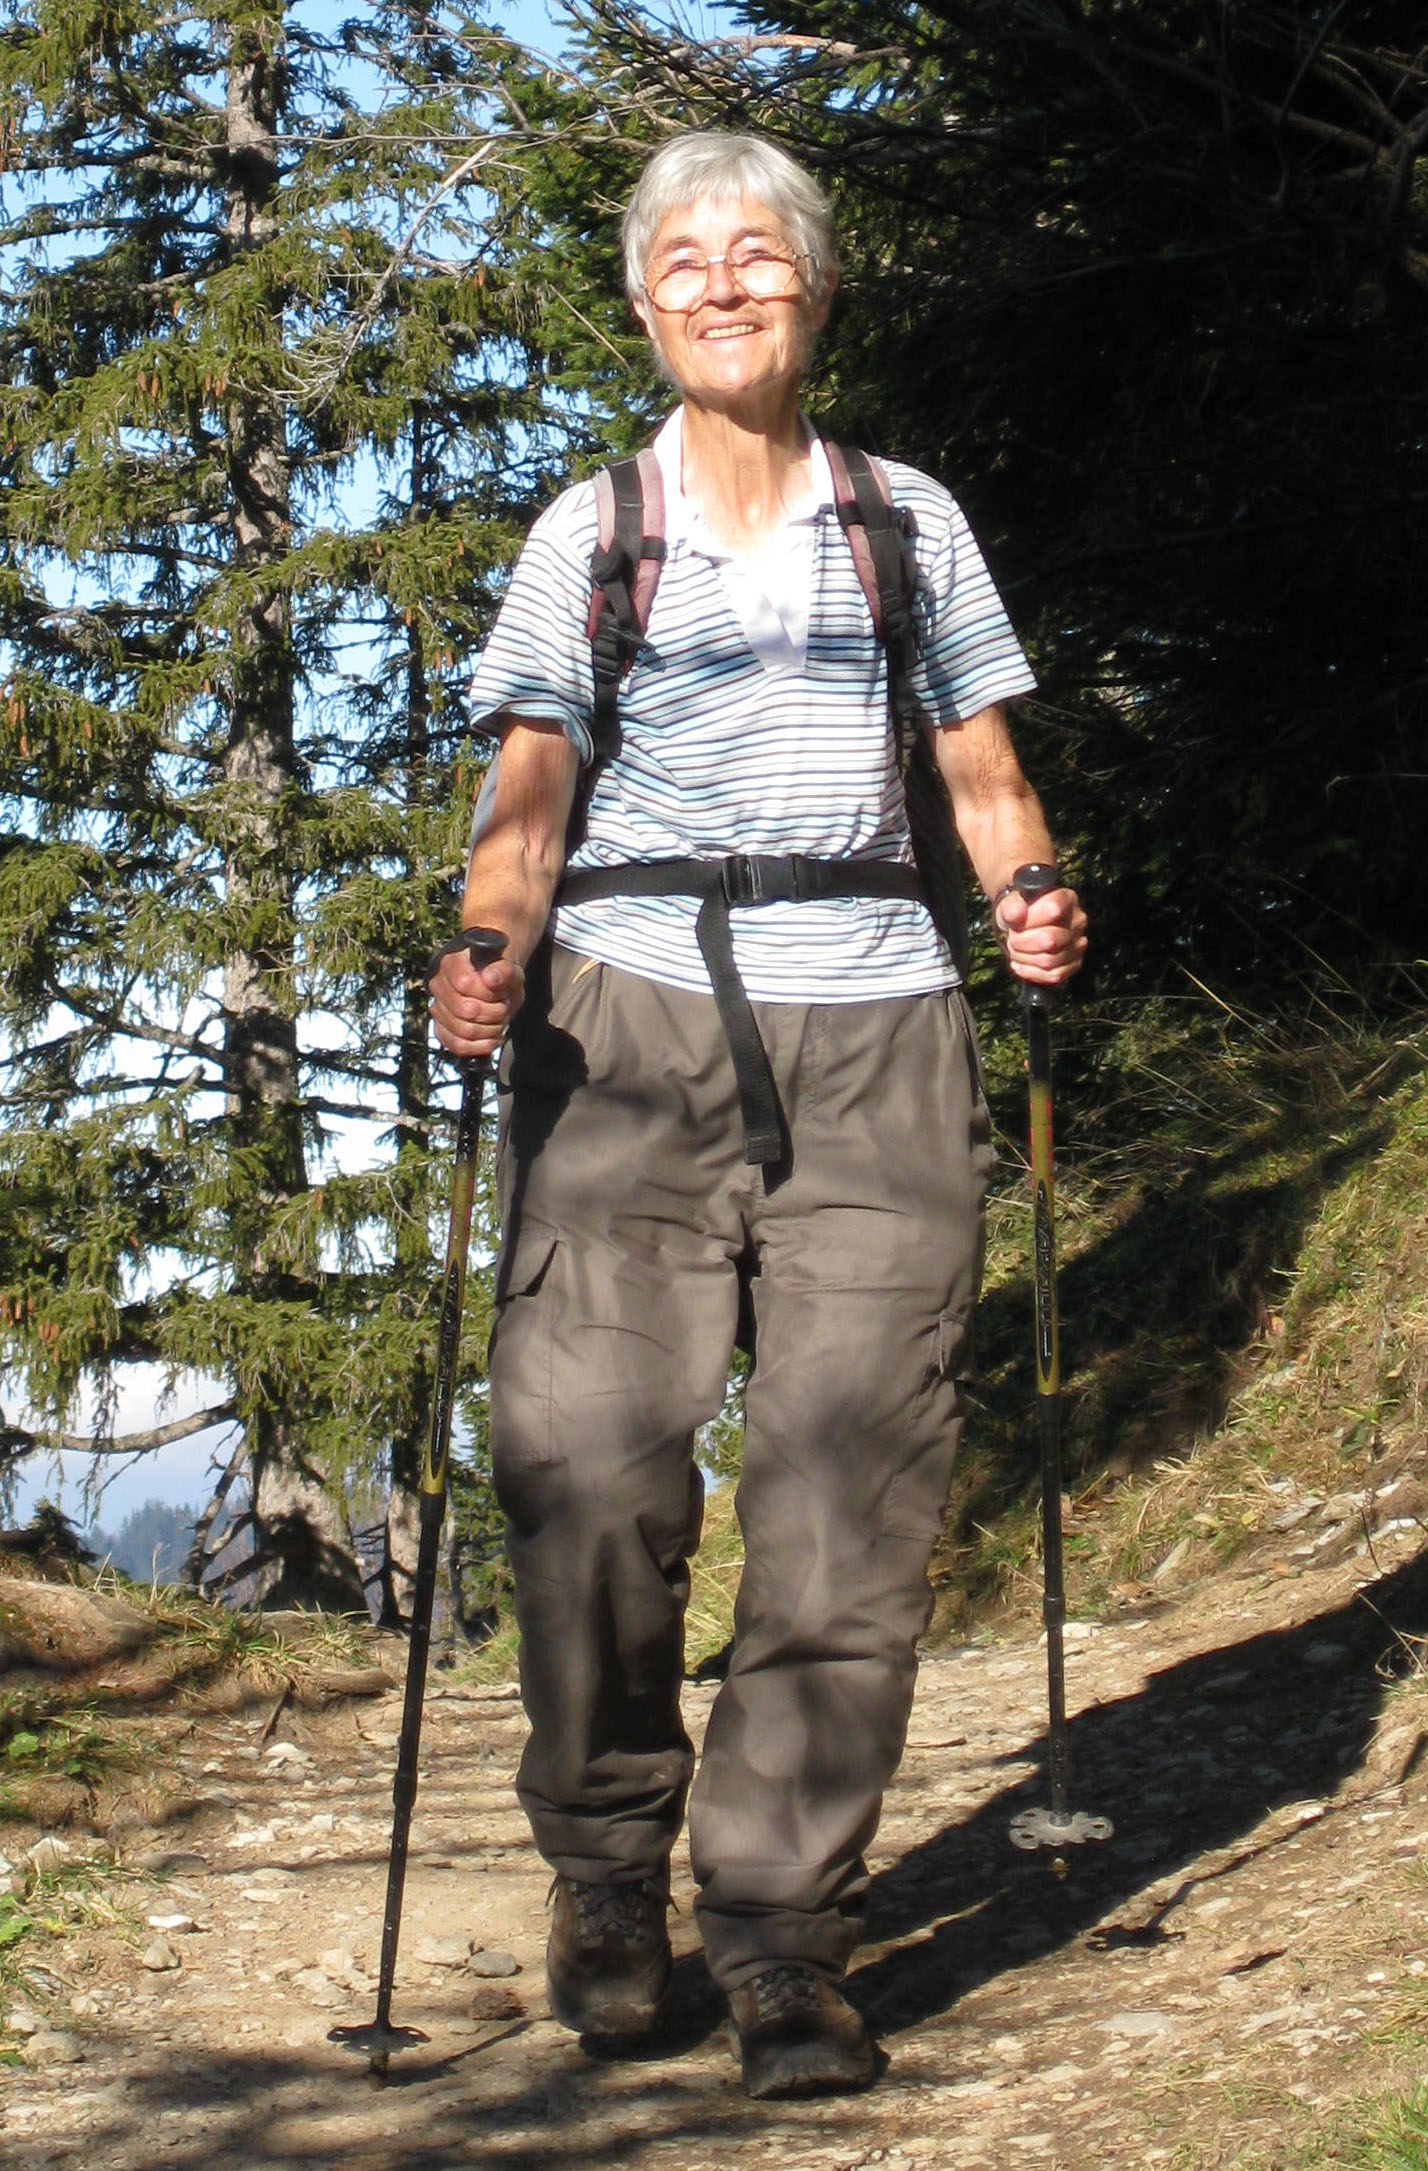
\includegraphics[width=0.8\textwidth]{figs/Iken_front_crop.jpg}
%\url{https://www.igsoc.org/awards/seligman/ikenseligman.html}
\end{column}
\begin{column}{0.5\textwidth}
\begin{itemize}
\item A is a glaciologist
\invisible<1>{\item she is not on a glacier, but happy to be hiking in the mountains}
\invisible<1-2>{\item she can say two \emph{precise} things about her patch of the world}
\invisible<1-3>{\item one equality and one inequality}
\invisible<1-4>{\item<5>[($=$)] the glacier thickness is zero
    $$H=0$$}

\vspace{-5mm}
\invisible<1-4>{\item<5>[($>$)] the mean annual surface mass balance is negative
    $$-a > 0$$}
\end{itemize}
\end{column}
\end{columns}
\end{frame}


\begin{frame}{two views in different patches}

\begin{columns}
\begin{column}{0.25\textwidth}
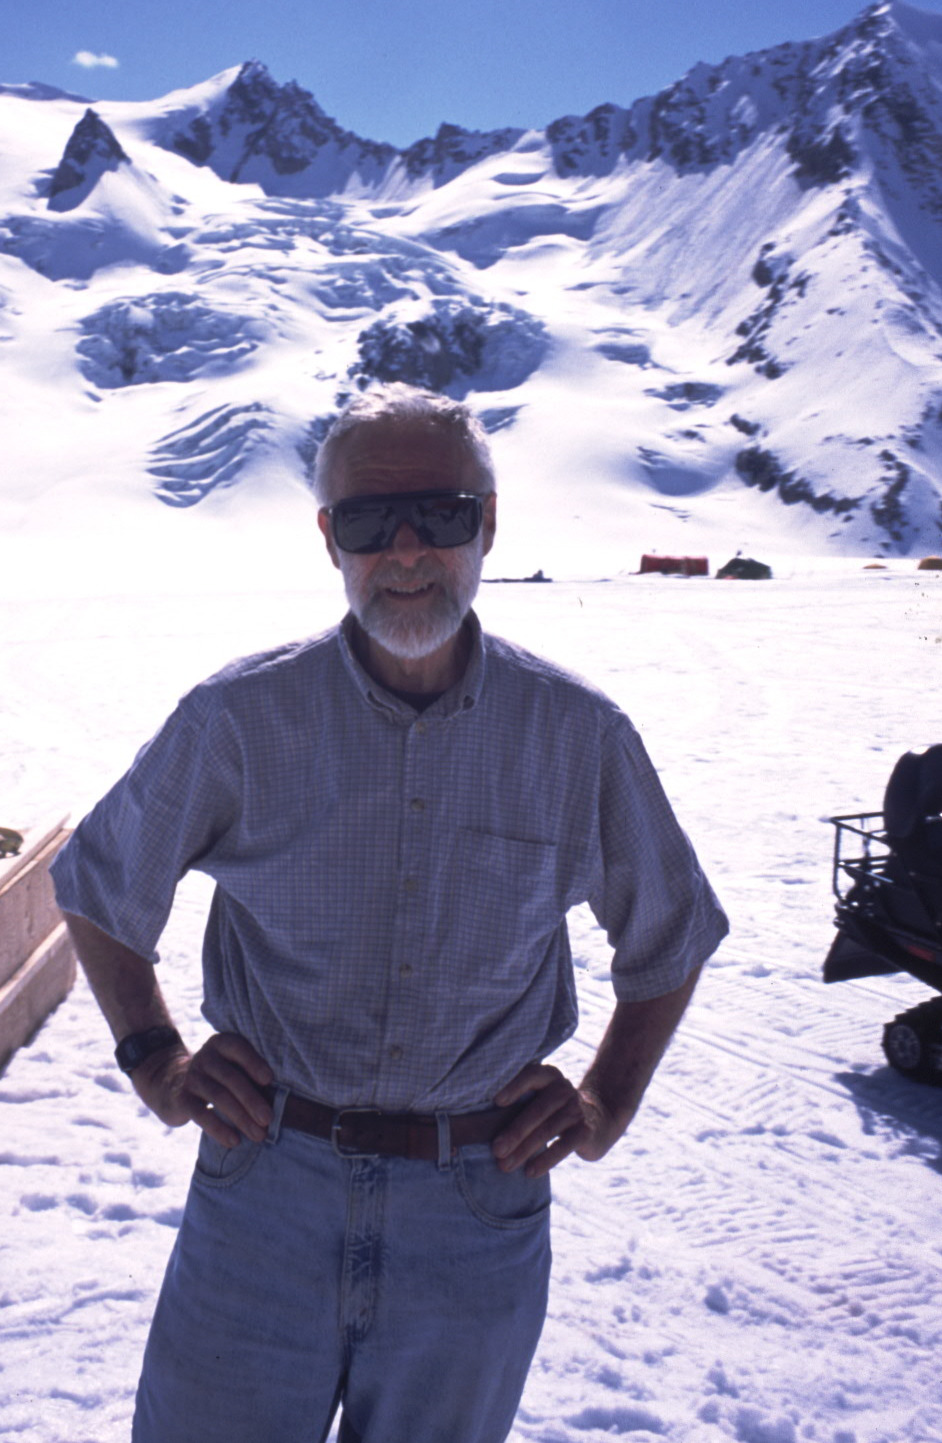
\includegraphics[width=0.75\textwidth]{figs/Will-by-Truffer.jpg}

\vspace{5mm}
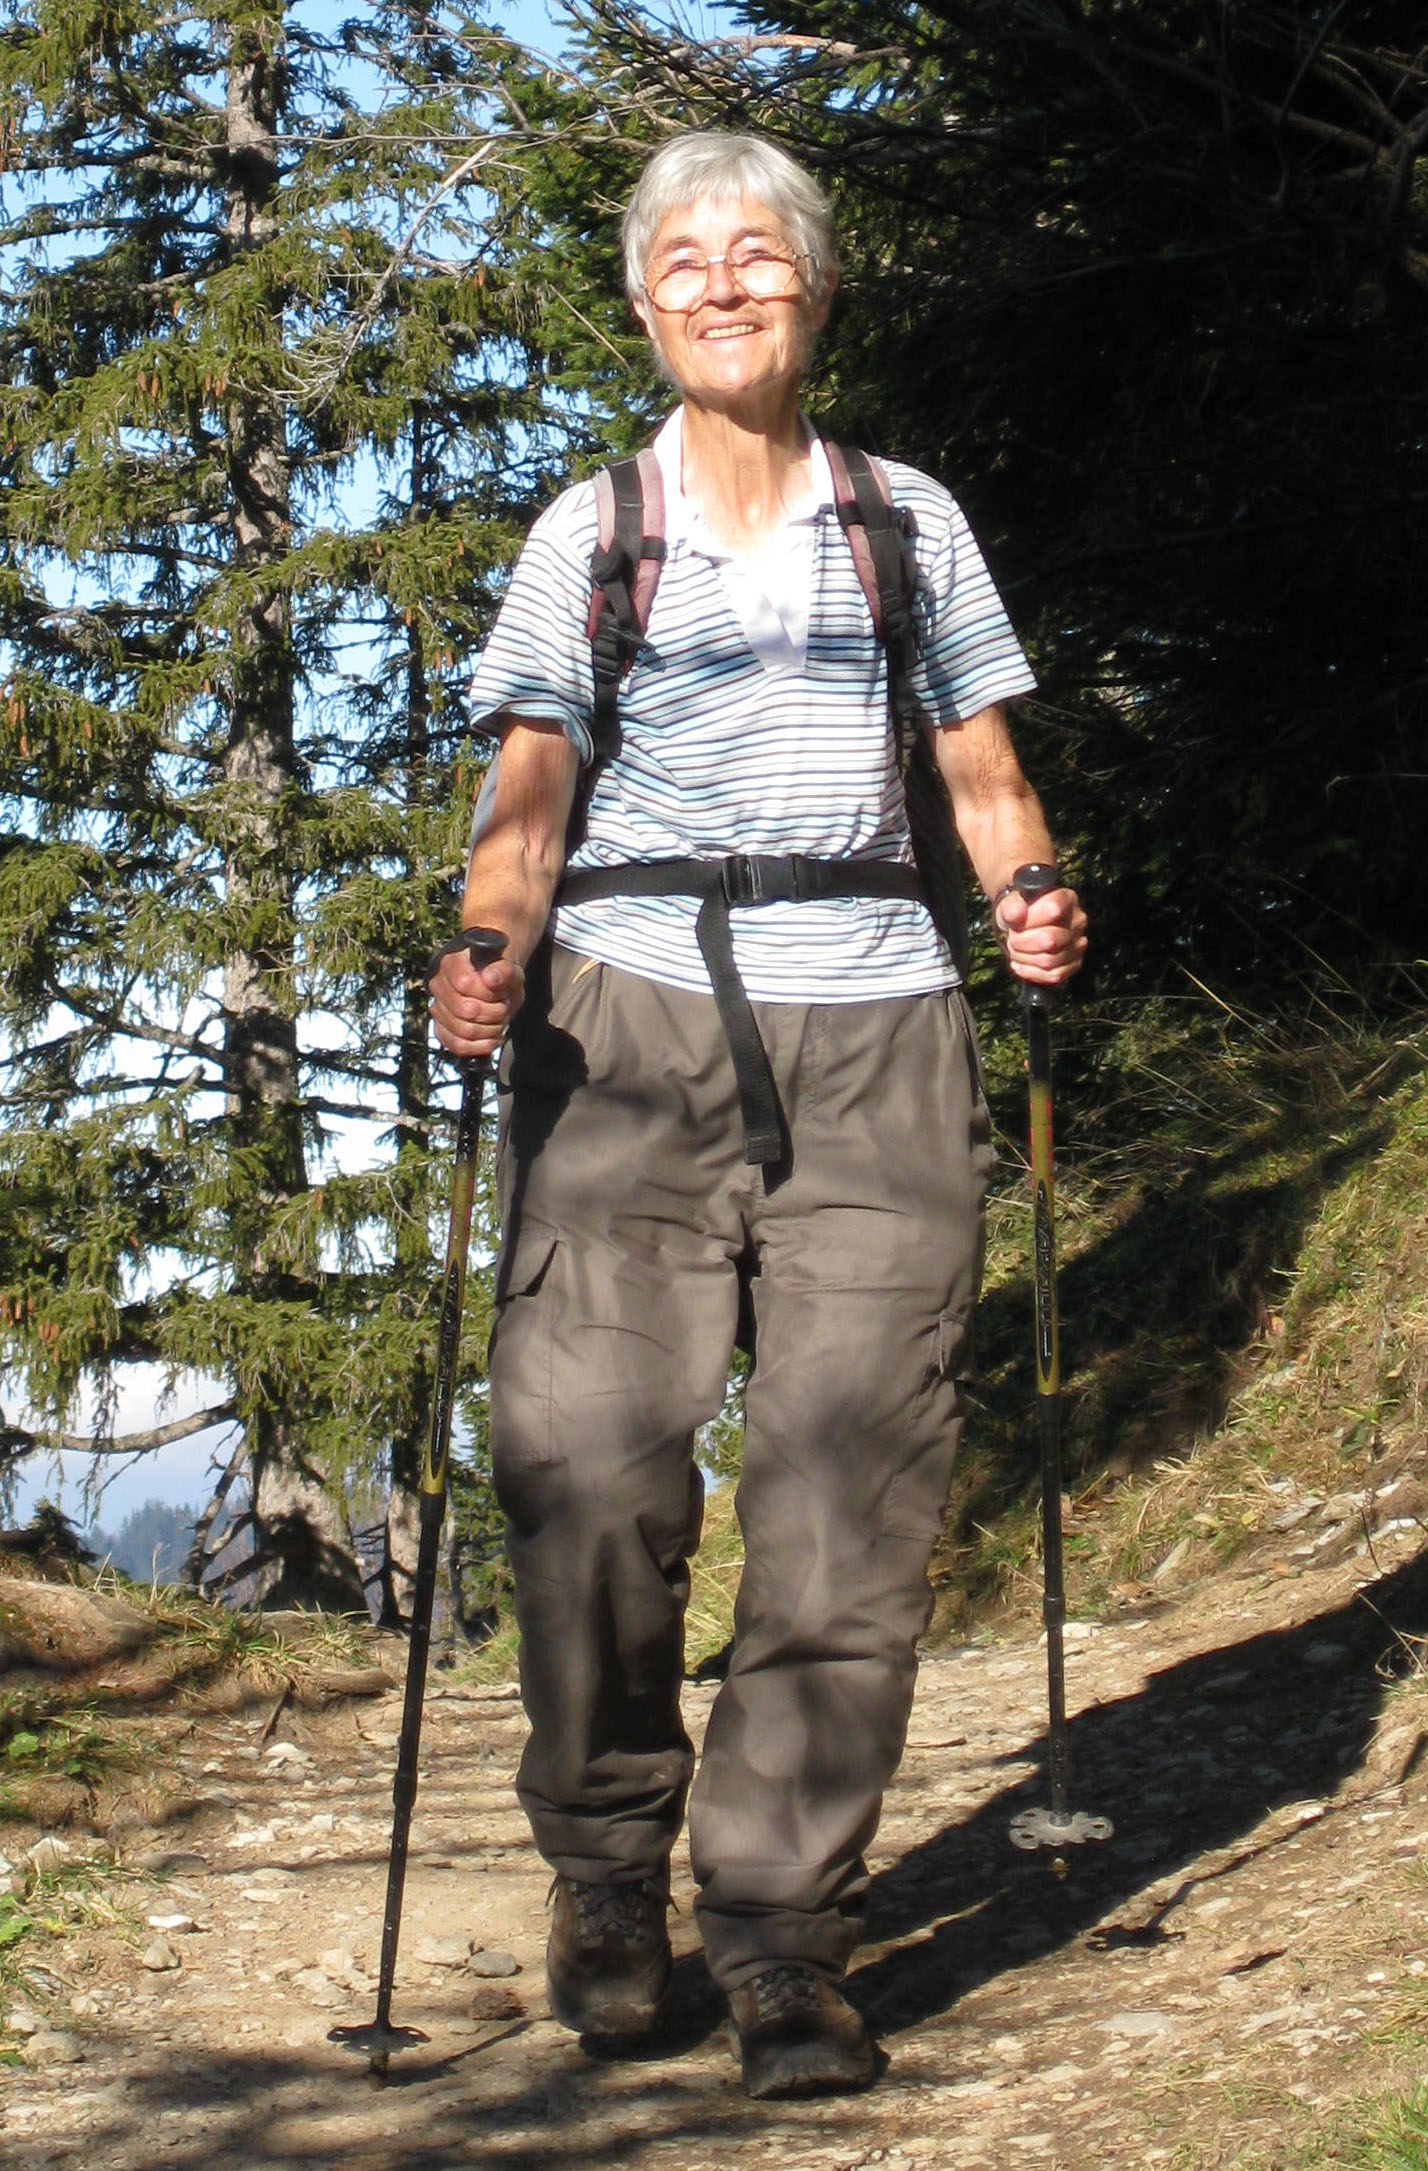
\includegraphics[width=0.75\textwidth]{figs/Iken_front_crop.jpg}
\end{column}
\begin{column}{0.75\textwidth}
\begin{itemize}
\item W says:
    \begin{itemize}
    \item[($>$)] the glacier thickness is positive
        $$H>0$$
    \item[($=$)] the mean annual surface mass balance is negative
        $$\frac{\partial H}{\partial t} + \Div \left(\bU H\right) = a$$
    \end{itemize}
\item A says:
    \begin{itemize}
    \item[($=$)] the glacier thickness is zero
        $$H=0$$
    \item[($>$)] the mean annual surface mass balance is negative
        $$-a > 0$$
    \end{itemize}
\item<2> so what?  the world looks different in different places!
\end{itemize}
\end{column}
\end{columns}
\end{frame}


\begin{frame}{define your terms}
\begin{itemize}
\item definitions!  please ask if you are unclear on some dumb symbol!

\bigskip
\item $\bx = (x,y)$ is map-plane location
\item $t$ is time \dots but much of this talk is about steady state

\medskip
\item $H(t,\bx)$ is glacier thickness
\item $b(\bx)$ is bed elevation
\item $s(t,\bx)$ is glacier surface elevation
\item $a(t,\bx)$ is annual surface (climatic) mass balance
\item $\bU = \bU(t,\bx)$ is vertically-averaged horizontal ice velocity
\item $\bu = \bu(t,x,y,z)$ is ice velocity \emph{in 3D}
\end{itemize}
\end{frame}


\begin{frame}{both views in one set of equations}
\begin{itemize}
\item xx
\end{itemize}
\end{frame}


\begin{frame}{xx}
\begin{itemize}
\item xx
\end{itemize}
\end{frame}


\section{complementarity for glaciers}

\begin{frame}{xx}
\begin{itemize}
\item xx
\end{itemize}
\end{frame}


\section{language from optimization}

\begin{frame}{xx}
\begin{itemize}
\item xx
\end{itemize}
\end{frame}


\section{consequences (for modelers and real scientists)}

\begin{frame}{xx}
\begin{itemize}
\item xx
\end{itemize}
\end{frame}

\begin{frame}{last}
\begin{itemize}
\item 
\item remembering Almut Iken (1933--2018) and Will Harrison (1936--2020)
\end{itemize}
\end{frame}


\end{document}

